\documentclass[tikz, convert={outext=.svg, command=\unexpanded{pdf2svg \infile\space\outfile}}, multi=false]{standalone}
\usepackage{tikz}

\usetikzlibrary{positioning, shapes, calc, shapes, arrows, decorations}

\tikzset{
	sigmoid/.style={
		path picture= {
    		\begin{scope}[x=1pt,y=10pt]
      			\draw plot[domain=-6:6] (\x,{1/(1 + exp(-\x))-0.5});
    		\end{scope}
    	}
	}	
}
\tikzset{
	relu/.style={
		path picture= {
    		\begin{scope}[x=1pt,y=1pt]
      			\draw plot[domain=-6:6] (\x,{max(0, \x)});
    		\end{scope}
    	}
  	}
}
\tikzstyle{hidden}=[draw,fill=gray!50,circle,minimum size=20pt,inner sep=0pt,relu]
\tikzstyle{outputNode}=[draw,fill=red!50,circle,minimum size=20pt,inner sep=0pt,sigmoid]
\tikzstyle{inputNode}=[draw,circle,minimum size=20pt,inner sep=0pt]
\tikzstyle{stateTransition}=[-stealth, thick]

\begin{document}
    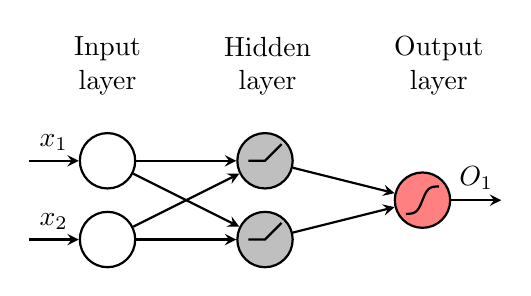
\begin{tikzpicture}
        \node[inputNode, thick] (i1) at (6, 1) {};
        \node[inputNode, thick] (i2) at (6, 0) {};

        \node[inputNode, thick, hidden] (h1) at (8, 1) {};
        \node[inputNode, thick, hidden] (h2) at (8, 0) {};


        \node[inputNode, thick, outputNode] (o1) at (10, 0.5) {};

        \draw[stateTransition] (5, 1) -- node[above] {$x_1$} (i1);
        \draw[stateTransition] (5, 0) -- node[above] {$x_2$} (i2);

        \draw[stateTransition] (i1) -- (h1);
        \draw[stateTransition] (i1) -- (h2);

        \draw[stateTransition] (i2) -- (h1);
        \draw[stateTransition] (i2) -- (h2);


        \draw[stateTransition] (h1) -- (o1);
        \draw[stateTransition] (h2) -- (o1);


        \node[above=1em of i1, align=center] (l1) {Input \\ layer};
        \node[right=2.3em of l1, align=center] (l2) {Hidden \\ layer};
        \node[right=2.3em of l2, align=center] (l3) {Output \\ layer};

        \draw[stateTransition] (o1) -- node[above] {$O_1$} (11, 0.5);


    \end{tikzpicture}
\end{document}